\documentclass[]{article}
\usepackage[nonatbib]{neurips_2021}
\usepackage[utf8]{inputenc}
\usepackage[T1]{fontenc}
\usepackage{amsfonts}
\usepackage{amsmath}
\usepackage{booktabs}
\usepackage{caption}
\usepackage{color}
\usepackage{courier}
\usepackage{graphicx}
\usepackage{adjustbox}
\usepackage{makecell}
\usepackage{microtype}
\usepackage{multirow,makecell}
\usepackage{nicefrac}
\usepackage{subcaption}
\usepackage{url}
\usepackage{xcolor}
\usepackage{hyperref}
\usepackage{cleveref}
\usepackage{xcolor,colortbl}
\usepackage{pgfplots}
\input{vedaldi}
\pgfplotsset{compat=1.17}

% No space paragraph.
\makeatletter
\renewcommand{\paragraph}{%
  \@startsection{paragraph}{4}%
  %{\z@}{3.25ex \@plus 1ex \@minus .2ex}{-1em}%
  {\z@}{0em}{-1em}%
  {\normalfont\normalsize\bfseries}%
}
\makeatother

% \DeclareMathOperator{\front_con}{Consistency_{front}}
% \DeclareMathOperator{\centre_con}{Consistency_{centre}}
% \DeclareMathOperator{\amin}{argmin}

% \title{Weakly-supervised 3D Object Detection by Automated Outlier Exclusion and Multi-View Consistency}
\title{Lifting 2D Object Locations to 3D by Discounting LiDAR Outliers across Objects and Views}
% \title{}
% \title{Lifting 2D Detections to 3D locations across multiple views}


\author{%
  David S.~Hippocampus\thanks{Use footnote for providing further information
    about author (webpage, alternative address)---\emph{not} for acknowledging
    funding agencies.} \\
  Department of Computer Science\\
  Cranberry-Lemon University\\
  Pittsburgh, PA 15213 \\
  \texttt{hippo@cs.cranberry-lemon.edu} \\
  % examples of more authors
  % \And
  % Coauthor \\
  % Affiliation \\
  % Address \\
  % \texttt{email} \\
  % \AND
  % Coauthor \\
  % Affiliation \\
  % Address \\
  % \texttt{email} \\
  % \And
  % Coauthor \\
  % Affiliation \\
  % Address \\
  % \texttt{email} \\
  % \And
  % Coauthor \\
  % Affiliation \\
  % Address \\
  % \texttt{email} \\
}

\begin{document}
\maketitle

\begin{abstract}
We present a system for automatic converting of 2D mask object predictions and raw LiDAR point clouds into full 3D bounding boxes of objects.
Because the LiDAR point clouds are partial, directly fitting bounding boxes to the point clouds is meaningless.
Instead, we suggest that obtaining good results requires sharing information between \emph{all} objects in the dataset jointly, over multiple frames.
We then make three improvements to the baseline.
First, we address ambiguities in predicting the object rotations via direct optimization in this space while still backpropagating rotation prediction through the model.
Second, we explicitly model outliers and task the network with learning their typical patterns, thus better discounting them.
Third, we enforce temporal consistency when video data is available.
With these contributions, our method significantly outperforms previous work despite the fact that these use significantly more complex pipelines, 3D models and additional human-annotated external sources of prior information.
% We propose a new direct optimization of the object rotations, fixing the ambiguity of the rotation estimation.
% Localising objects in 3D is a fundamental requirement of many robotic systems. This task requires a large amount of annotated training data which is expensive to obtain and of questionable accuracy for some objects. In contrast 2D annotations are much simpler to obtain and train as has been shown in many recent works. In this work we propose a method which allows the use of a pre-trained 2D instance segmentation network to train a 3D object detection network without the need for expensive 3D annotations. The main contributions of our method are as follows: 1) automatic segmentation of raw LiDAR data by learning to remove outlier points during training 2) novel training scheme that avoids local optima in viewpoint estimation 3) learning across multiple frames that enforces temporal consistency of the scene. Our method significantly outperforms previous yet more complex methods while also requiring less supervision for training.
%The method automatically segments raw LiDAR data by learning to remove outlier points during training and by combining it with novel training scheme which avoids local optima and with enforcing scene consistency between multiple frames, the method significantly outperforms previous yet more complex methods.
\end{abstract}

\section{Introduction}\label{s:introduction}

Robotics applications often require to recover the 3D shape and location of objects in world coordinates.
This explains the proliferation of datasets such as KITTI, nuScenes and SUN RGB-D~\cite{geiger12are-we-ready,nuscenes2019,sun2020scalability} which allow to train models that can classify, detect and reconstruct objects in 3D from sensors such as cameras and LiDARs.
However, creating such datasets is very expensive.
For example,~\cite{sun-rgbd,wang2019apolloscape} report that manually annotating a single object with a 3D bounding box requires approximately 100 seconds.
While this cost has since been reduced~\cite{meng2020ws3d}, it remains a significant bottleneck in data collection.

\begin{figure}[h]
    \centering
    \begin{tabular}{c c}
        \includegraphics[width=0.5\textwidth]{figures/Qualitative_examples/411.png} & 
        \includegraphics[width=0.5\textwidth]{figures/Qualitative_examples/50.png} \\
         
        % \includegraphics[width=0.5\textwidth]{figures/Qualitative_examples/172.png} & 
        % \includegraphics[width=0.5\textwidth]{figures/Qualitative_examples/52.png} \\
        
        % \includegraphics[width=0.5\textwidth]{figures/Qualitative_examples/171.png}
        %  &  \includegraphics[width=0.5\textwidth]{figures/Qualitative_examples/241.png} \\
 

        
    \end{tabular}
    \caption{Our Method (green) vs KITTI label (red), no Ground Truth is used to train our model. }
    \label{f:Qualitative}
\end{figure}
In some cases, cross-modal learning can substitute manual annotations.
% for one sensor, such as a camera, can be obtained automatically from a different sensors, such as  LiDAR\@.
An example is monocular depth prediction, where supervision from a LiDAR sensor is generally sufficient~\cite{Fu_2018_CVPR}.
Unfortunately, this does not extend to tasks such as object detection.
For instance, a dataset such as KITTI provides only $7481$ video frames annotated with objects due to the cost of manual annotation.
% LiDAR information is still used to allow annotators to determine the location of the objects in 3D space.
% However, many object occurrences are small and partially occluded, resulting in few LiDAR points per object instance and thus increasing the difficulty of obtaining correct manual annotations~\cite{feng2020labels}.
In this work, we thus consider the problem of detecting objects in 3D, thus also automatically annotating them in 3D, but using only standard 2D object detector trained on a generic dataset such as MS-COCO~\cite{lin2014microsoft}, which is disjoint from the task-specific dataset (in our case KITTI for 3D car detection).
We assume to have as input a collection of video frames, the corresponding LiDAR readings from the viewpoint of a moving vehicle, and the ego-motion of the vehicle.
We also assume to have a pre-trained 2D detector and segmenter such as Mask R-CNN\@ for the objects of interest (e.g., cars).
With this information, we wish to train a model which takes in raw LiDAR point cloud and outputs full 3D bounding box annotation for the detected objects without incurring any further manual annotation cost.

% As discussed above, this problem is rather challenging, but solving it can significantly reduce the data annotation cost and therefore allow to obtain richer and more representative labelled datasets for robotics applications.
% Because of the applicative potential, we are not the first to consider this challenge.
% For instance, the authors of~\cite{sdflabel} recently proposed a sophisticated approach for auto-labelling that uses a combination of differentiable rendering, synthetic pretraining, and canonical maps using a sign-distance-function (SDF) representation.
% The authors of~\cite{qin20weakly} proposes instead a method that combines an heuristic 3D bounding box proposal step and then learn to filter them to be compatible with the available 2D annotations.

There are three main challenges.
First, due to self and mutual occlusions, the LiDAR point clouds only cover part of the objects in a context dependent manner.
Second, the LiDAR readings are noisy, for example sometimes seeing through glass surfaces (windows) and sometimes not.
Third, the available 2D segmentations may not be perfectly semantically aligned with the target class (e.g., `vehicles' vs `cars'), are affected by a domain shift, and may not be perfectly geometrically with the LiDAR data, resulting in a large number of outlier 3D points arising from background objects.
%  that 3D points in the background can also be included in the estimate, significantly skewing any direct bounding box fit.

We propose an approach based on the following key ideas.
First, because the LiDAR point cloud can only cover the object partially, it is impossible to estimate the full 3D extent of the object from a single observation of it.
Instead, we share information between all predicted 3D boxes in the dataset by \emph{learning a 3D bounding box predictor from all the available data}.
%{\color{red} Learning the predictor is a means rather than an end:} the goal is to \emph{share information} between the thousands of object instances that exist in the dataset to obtain predictions that are overall consistent.
We further aid the process by injecting weak prior information in the form of a single fixed 3D mesh template of the object (an `average car'), but avoid sophisticated 3D priors employed in prior works~\cite{sdflabel,qin20weakly}.

We then introduce three improvements to the `obvious' baseline implementation of this idea.
First, we show that a key challenge in obtaining good 3D bounding boxes is to estimate correctly the yaw (rotation) of the object.
This is particularly challenging for partial point clouds as several ambiguous fits (generally up to rotations of 90 degrees) often exist.
Prior work has addressed this problem by using pre-trained yaw predictors, requiring manual annotation.
Here, we learn the predictor automatically form the available data only.
To this end, we show that mere local optimization via gradient descent works poorly;
instead, we propose to systematically explore a full range of possible rotations for each prediction, backpropagating the best choice every time.
We show that this selection process is very effective at escaping local optima and results in excellent, and automated, yaw prediction.

Second, we note that the LiDAR data contains significant outliers.
We thus propose to automatically learn the \emph{pattern} of such outliers by predicting a confidence score for each 3D point, treated as a Gaussian observation.
These confidences are self-calibrated using a neural network similar to the ones used for point cloud segmentation, configured to model the aleatoric uncertainty of the predictor.

Third, we note that we generally have at our disposal \emph{video data}, which contains significant more information than instantaneous observations.
We leverage this information by enforcing a simple form of temporal consistency across several frames.

As a result of these contributions we obtain a very effective system for automatically labelling 3D objects.
Our system is shown empirically to outperform relevant prior work by a large margin, all the while being simpler, because it uses less sources of supervision and because it does \emph{not} use sophisticated prior models of the 3D objects nor a large number of 3D models as priors~\cite{sdflabel,qin20weakly}

% In this work, we suggest an alternative approach that directly lifts 2D annotations in 3D.
% Given a 2D bounding box annotation and the corresponding object mask from Mask R-CNN, we first select the LiDAR points that fall within this region.
% This results in a noisy collection of 3D points, part of which correspond to the target object (inliers), and part to the background or other objects (outliers).
% Then, we fit to these LiDAR points to an `average' car template (a simple off-the-shelf 3D mesh) by minimizing a fitting loss, thus obtaining the location of the object in 3D.

% While this simplistic approach fails to generate satisfactory results, we introduce two ideas that substantially improve its performance.
% The first idea is to avoid minimizing the fitting loss directly;
% instead, we learn a neural network that, given a point cloud as input, produces as output the parameters of the fit.
% Since this network is trained using the same fitting loss and data samples as before, it is not immediately obvious why this should bring any benefits.
% The reason, we show, is that the network can pool information across \emph{all} object instances in the dataset in order to fit each individual instance.
% In other words, by observing the samples collection as a whole, the network extracts a data prior.
% By leveraging this prior, it can obtain much better fits for those object instances for which the LiDAR evidence is noisy, ambiguous or scarce.

% A second significant issue is the presence of outliers in the data.
% For the most part, outliers are LiDAR points that are incorrectly assigned to the target object due to imperfections in the Mask R-CNN detection.
% This is particularly serious when, as it is often the case, several objects partially overlap, because the algorithm may just decide to fit the incorrect object instance.
% We address this issue by extending our fitting network with the ability to predict a confidence that individual LiDAR points are inliners with respect to the selected target object.
% We cast this as a probabilistic observation model, and task the network to predict a per-point fitting variance.
% The resulting probabilistic loss function is self-calibrated and effectively learns to distinguish inliers from outlier.

% We show empirically that our approach is considerably simpler than~\cite{sdflabel}, while achieving superior accuracy.


\section{Related work}\label{s:related}

%sdf skips annotation when Mask-rcnn box less than 50% of GT 
%https://github.com/TRI-ML/sdflabel/blob/master/pipelines/refine_css.py line 110
%line 186 seems t change estimate of height based on how good the iou of the model is vs rcnn/gt box

% \paragraph{Object Detection in 2D} %??.?

\paragraph{Supervised.}

3D object detection methods assume availability of either monocular RGB images, LiDAR point clouds or both. Here we focus on supervised methods using 3D point cloud inputs. \cite{wang2015voting,engelcke2017vote3deep} discretise point clouds onto a sparse 3D feature grid and apply convolutions while excluding empty cells. \cite{chen2017multiview} project the point cloud onto the frontal and the top views, apply 2D convolutions thereafter and generate 3D proposals with an RPN \cite{ren16faster}. \cite{zhou2018voxelnet} convert the input point cloud into a voxel feature grid, apply a PointNet \cite{qi16pointnet:} to each cell and subsequently process it with a 3D fully convolutional network with an RPN head which generates object detections.
Frustum PointNets \cite{qi2017frustum} is a two step detector which first detects 2D bounding boxes using these to determine LiDAR points of interest which are filtered further by a segmentation network. The remaining points are then used to infer the 3D box parameters with the centre prediction being simplified by some intermediate transformations in point cloud origins. We are using Frustum PointNets as a backbone for our method.

\paragraph{Weakly Supervised.}

Owing to the complexity of acquiring a large scale annotated dataset for 3D object detection many works recently have attempted to solve this problem with less supervision. \cite{meng2020ws3d} the required supervision is reduced from the typical $(X,Y,Z)$ centre, $yaw$, $(x_1,y_1,x_2,y_2)$ 2D box and $(l,w,h)$ 3D size they instead annotate 500 frames with centre $(X,Z)$ in the Birds Eye View and finely annotating a 534 car subset of these frames to achieve accuracy similar to models trained on the entire Kitti training set. This however can result in examples in the larger training set or validation set which are outside the distribution of cars seen in the smaller subset, are also susceptible to the problems mentioned in \cite{feng2020labels} and the weakly annotated centres can have a large difference to the Kitti annotations. In \cite{sdflabel} trains DeepSDF\cite{Park_2019_CVPR} on models from a synthetic dataset which are then rendered into the image and iteratively refined to produce a prediction that best fits the predictions of Mask R-CNN outputs.
% {\color{red} (which are sufficiently close to ground truth 2D boxes)}. 
This however takes 6 seconds to refine predictions on each input example and ground truth 2D boxes are used to select cars used to train on. In \cite{qin20weakly} 3D anchors densely placed across the range of annotations are projected into the image with object proposed by looking at the density of points within or nearby the anchors in 3D and the 3D pose and 2D detections are supervised by a CNN trained on Beyond PASCAL\cite{xiang14beyond}. In \cite{koestler2020learning} instance segmentation is used to place a mesh in the location of detected cars which is refined using supervised depth estimation. 

\paragraph{Viewpoint estimation.}
Estimating 3D camera orientation is an actively researched topic \cite{pepik12teaching, kendall2015posenet, tulsiani15viewpoints, su2015render, mousavian20173d, prokudin2018deep, liao2019spherical}. Central to this problem is the choice of an appropriate representation for rotations. Directly representing rotations as angles $\theta \in [0, 2\pi )$ suffers from discontinuity at $2\pi$. One way to mitigate this is to use the trigonometric representation $(\cos \theta, \sin \theta)$ \cite{penedones2012improving, massa2016crafting, beyer2015biternion}. Another approach is to discretise the angle into $n$ quantised bins and treat viewpoint prediction as a classification problem \cite{tulsiani15viewpoints, su2015render, mousavian20173d}. Quaternions are another popular representation of rotations used with neural networks \cite{kendall2015posenet, xiang2017posecnn}. Learning camera pose without direct supervision, for example, when fitting a 3D model to 2D observations, may suffer from ambiguities due to the object symmetries \cite{saxena2009learning}. Practically, this means that the network can get stuck in a local optima of $SO(3)$ space and not be able to recover the correct orientation. Several recent works \cite{tulsiani2018multi, insafutdinov18pointclouds, goel20shape} overcome this by maintaining several diverse candidates for the estimated camera rotation and selecting the one that yields the best reconstruction loss. Our approach discussed in sec.~\ref{s:direct-yaw} is most related to these methods.

%Predicting Yaw as one of $n$ quantised steps is well studied approach in supervised learning approaches. Compared to continuous predicted values in the vector and quaternion approaches this does not have an issue with the discontinuity present at the jump between $0$ and $2\pi$ where the the loss value is quite high but the actual error is relatively quite small.} 
\newcommand{\X}{\mathbf{X}}
\section{Method}\label{s:method}

\begin{figure}
\centering
%\includegraphics[width=0.75\textwidth]{figures/method/FPN.png}
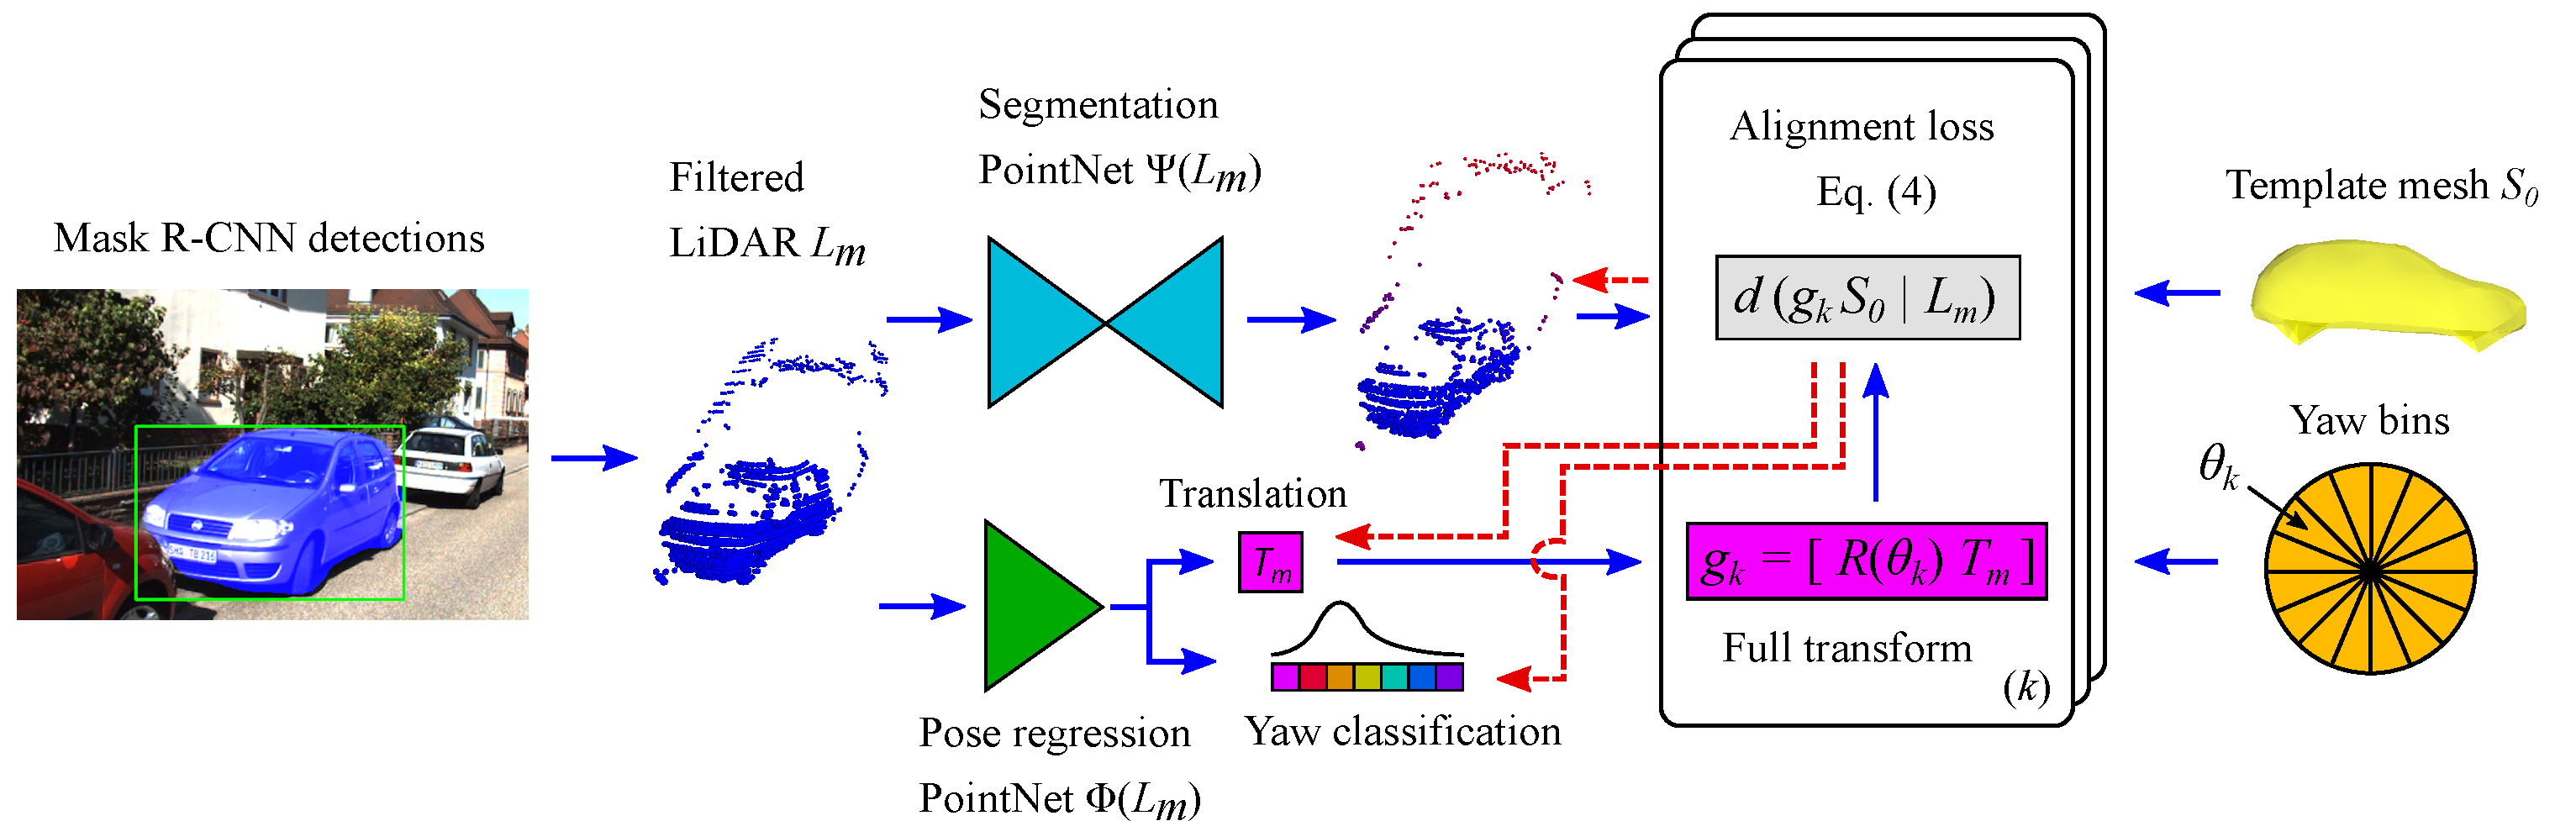
\includegraphics[width=1.0\textwidth]{figures/system.pdf}
\caption{Network architecture. Dashed arrows in red show the flow of the gradients during the backward pass. Alignment loss is evaluated for each yaw bin $\theta_k$ and the optimal yaw is used to supervise the yaw classification network $\Phi_r$ (see sec.~\ref{s:direct-yaw}).}\label{fig:network_architecture}
% source: system.svg created in Inkscape
% https://drive.google.com/file/d/1hjJ9znYa3mIgfydyCUSzDMKnB1lmoKT3/view?usp=sharing
\end{figure}

Our goal is to estimate the 3D bounding box of objects given as input videos with 2D mask predictions and LiDAR point clouds.
We discuss first how this problem can be approached by direct fitting and then develop a much better learning-based solution.

\subsection{Shape model fitting}\label{s:shapemodel}

We first describe how a 3D bounding box can be fitted to the available data in a direct manner.
To this end, let $I \in \mathbb{R}^{3\times H\times W}$ be a RGB image obtained from the camera sensor and let $L \subset\mathbb{R}^3$ be a corresponding finite collection of 3D points $\X\in L$ extracted from the LiDAR sensor.
Furthermore, let $m \in \{0,1\}^{H \times W}$ be the 2D mask of the object obtained from a system such as Mask R-CNN~\cite{he17mask} from image $I$.
Our goal is to convert the 2D mask $m$ into a corresponding 3D bounding box $B$.

To do so, assume that the LiDAR points are expressed in the reference frame of the camera and that the camera calibration function $k : \mathbb{R}^2 \rightarrow \Omega = \{1,\dots,H\}\times\{1,\dots,W\}$ is known.
The calibration function is defined such that the 3D point $\X=(X,Y,Z)$ projects onto the image pixel $u = k(\pi(\X))$ where $\pi(X,Y,Z)=(X/Z,Y/Z)$ is the perspective projection.
In particular, the subset of LiDAR points $L_m \subset L$ that project onto the 2D mask $m$ is given by:
$
L_m
=
L \cap
(k \circ \pi)^*(m)
$
where ${}^*$ denotes the pre-image of a function.
In practice, this is a crude filtering step, because the masks are imprecise and not perfectly aligned to the LiDAR and because LiDAR may sometimes see `through' the object, for instance in correspondence of glass surfaces
% as one point of the mask $m$ in the pixel space obviously potentially corresponds to an infinite number of 3D LiDAR points; this property manifests in practice by including 3D LiDAR points which are in front of the vehicle as well as LiDAR points behind the actual object, as for example car windows are transparent to LiDAR
(see \cref{fig:dataset_example}).

\begin{figure}
    \centering
    \begin{tabular}{c c c c}
         \includegraphics[width=0.25\textwidth]{figures/method/examples/rgb-2.png}
        &\includegraphics[width=0.2\textwidth]{figures/method/examples/pcd-2.png} &
         \includegraphics[width=0.2\textwidth]{figures/method/examples/rgb-4.png}
        &\includegraphics[width=0.2\textwidth]{figures/method/examples/pcd-4.png} \\
    \end{tabular}
    \caption{
    For each pair, left: RGB input image with Mask R-CNN predicted box and highlighted pixels inside the mask.
    Right: LiDAR points in blue represent those inside the 2D mask, green those outside.
    Note that, while the image mask removes many outliers, not all of them ares.}\label{fig:dataset_example}
\end{figure}


In order to fit a 3D bounding box $B$ to $L_m$, we use a weak prior on the 3D shape of the object.
Specifically, we assume that a 3D template surface $S_0\subset\mathbb{R}^3$ is available, for example as simplicial (triangulated) mesh.
We fit the 3D surface to the LiDAR points by considering a rigid motion $g \in SE(3)$ which, applied to $S_0$, results in the posed mesh
$
S = gS_0 = \{g\X : \X \in S_0\}.
$
We then define a distance between the mesh and the 3D LiDAR points as follows:
\begin{align}\label{e:dist1}
d(S|L_m)
&=
\frac{1}{|L_m|}
\sum_{\X \in L_m}
\min_{\X' \in S}
\|\X' - \X \|^2.
\end{align}
This quantity is similar to a Chamfer distance, but it only considers half of it:
this is because most of the 3D points that belong to the template object are \emph{not} be visible in a given view (in particular, at least half are self-occluded), so not all points in the template mesh have a corresponding LiDAR point.

% While~\cref{e:dist1} can be computed exactly if $S$ is a mesh, in practice we found it beneficial to replace this quantity with the following `noisy estimate':
% \begin{align}\label{e:dist2}
%   \hat d(S|L_m)
%   &=
%   E_{\hat S}\left[
%   \frac{1}{|L_m|}
%   \sum_{\X \in L_m}
%   \min_{\X' \in \hat S}
%   \|\X' - \X \|^2
%   \right]
% \end{align}
% where $\hat S$ is a finite collection of 3D points sampled uniformly at random on the surface $S$ of the object (in the experiment, we set $|\hat S| = 1000$).
% In addition to making the calculation of~\cref{e:dist1} faster, using \cref{e:dist2} in a stochastic optimizer might help convergence by escaping local optima.

Given a 2D object mask $m$ and its corresponding LiDAR points $L_m$, we can find the pose $g$ of the object by minimizing $d(g S_0|L_m)$ with respect to $g \in SE(3)$.
Then the bounding box of the object $m$ is given by $gB_0$ where $B_0 \subset \mathbb{R}^3$ is the 3D bounding box that tightly encloses the template $S_0$.

In accordance with prior work~\cite{geiger12are-we-ready,qin20weakly,meng2020ws3d}, we can in practice carry out the minimization not over the of full space $SE(3)$, but only on 4-DoF transformation $g = [R_\theta,~\mathbf{T}]$ where the rotation $R_\theta$ is restricted to the \emph{yaw} $\theta$ (rotation perpendicular to the ground plane).
Even so, direct minimization of~\cref{e:dist1} is in practice prone to failure because individual partial LiDAR point clouds do not contain sufficient information and fitting results are thus ambiguous (we do not report results in this setting as they are extremely poor).

%\subsection{Learning-based fitting}\label{s:model}

% Because directly fitting~\cref{e:dist2} to a small set of LiDAR points that only observe a fraction of the surface $S_0$ is ambiguous and works poorly due to noise and occlusions ({\color{red} see ablation experiment}),

Our solution to the ambiguity of fitting~\cref{e:dist1} is to \emph{share information} across all object instances in the dataset.
We do this by training a deep neural network
$
\Phi : \operatorname{Fin}(\mathbb{R}^3) \rightarrow SE(3)
$
mapping the LiDAR points $L_m$ to the corresponding object pose $g = \Phi(L_m)$ directly.
The network $\Phi$ can be trained in a self-supervised manner by minimizing \cref{e:dist1} averaged over the entire dataset
$
\mathcal{D}
$
as
\begin{align}\label{e:simpleloss}
  %  (R_m, \mathbf{T}_m) &= \Phi(L_m) \\\label{e:simpleloss}
  \mathcal{L}(\Phi|\mathcal{D})
  &=
  \frac{1}{|\mathcal{D}|}
  \sum_{(L_m,m)\in\mathcal{D}}
  d(g_m S_0 | L_{m}),
  ~~~
  \text{where} ~ g_m = \Phi(L_m).
\end{align}
%{\color{red}Note that our goal is not so much to train the predictor $\Phi$ (although this is also useful), but rather to obtain the fits $g_m=[R_{\theta_m}~ \mathbf{T}_m] = \Phi(L_m)$.}
% The network is an auxiliary byproduct of this process.
% In particular, note that we retain the output of the network on the dataset $\mathcal{D}$ (which would normally be discarded as this is also the training set) -- this is a form of self-supervision.

\subsection{Modelling and discounting outliers}

% \begin{figure}
    \centering
    \begin{tabular}{c c c c}

        %  \includegraphics[width=0.2\textwidth]{figures/method/ambiguous/ex2/rgb.png}
        % &\includegraphics[width=0.2\textwidth]{figures/method/ambiguous/ex2/pcd.png} &
         \includegraphics[width=0.2\textwidth]{figures/method/ambiguous/ex3/rgb.png}
        &\includegraphics[width=0.1\textwidth]{figures/method/ambiguous/ex3/pcd.png} &
         \includegraphics[width=0.2\textwidth]{figures/method/ambiguous/ex5/rgb.png}
        &\includegraphics[width=0.2\textwidth]{figures/method/ambiguous/ex5/pcd.png}
        
    \end{tabular}
    
    \caption{Even with the pixel level Mask-RCNN detections our remaining pointclouds in blue can still have a lot of noise caused occluding objects or imperfect masks which cause problems for a chamfer distance like fit}
    \label{fig:dataset_example}
    
\end{figure}
\begin{figure}
    \centering
    
        
        \begin{tabular}{c c c c}
            \includegraphics[width=0.25\textwidth]{figures/method/output_examples/rgb-1.png} &
            \includegraphics[width=0.25\textwidth]{figures/method/output_examples/pcd-1.png} &
            \includegraphics[width=0.25\textwidth]{figures/method/output_examples/rgb-2.png} &
            \includegraphics[width=0.25\textwidth]{figures/method/output_examples/pcd-2.png}
        \end{tabular}
        \caption{Even after removing LiDAR points which do not project into the 2D instance mask we still have a large number of outliers, mainly caused by partial occlusions and points at the boundary where 2D masks struggle. The $\sigma^2(\X)$ value predicts the relevance of a point to the cars location with blue points having low values with a gradient to red for higher values which suggests the point is an outlier.}
    \label{fig:my_label}
\end{figure}

A major drawback of~\cref{e:simpleloss} is that LiDAR points tend to be noisy, especially because the boundaries of the region $m$ may not correspond to the object exactly or the LiDAR may be affected by a reflection or `see through' a glass surface.
Such points might disproportionally skew the loss term, forcing the estimated object position closer to these outliers.
In order to help the model discriminate between inliers and outliers, we let the network predict an estimate of whether a given measurement is likely to belong to the object or not.

We therefore propose a second network $\sigma(\X) = \Psi_\X(L_m)$ that assigns to each LiDAR point $\X \in L_m$ a variance $\sigma$ and jointly optimize $\Phi$ and $\Psi$ by minimizing~\cite{novotny17learning,kendall17what}:
\begin{equation}\label{e:distance}
  \bar d(S|L_m)
  =
  %E_{\hat S}\left[
  \frac{1}{|L_m|}
  \sum_{\X \in L_m}
  \min_{\X' \in \hat S}
  \frac{\|\X' - \X \|^2}{\sigma^2(\X)}
  +
  \log \sigma^2(\X)
  %\right]
  % \label{e:sigmaloss}
  %  \mathcal{L}''(\Phi, \Psi|\mathcal{D})
  % &=
  % \frac{1}{|\mathcal{D}|}
  % \sum_{(L_m,m)\in\mathcal{D}}
  % \bar d(g_m S_0 | L_{m}).
\end{equation}
Note that the network $\Psi$ has to make a judgement call for every point $\X$ on whether it is likely to be an outlier or not \emph{without} having access to the loss.
A perfect prediction (i.e., one that minimizes the loss) would set $\sigma(\X) = \|\X' - \X \|$ to be the same as the fitting error.
The desirable side effect is that, in this manner, outliers are discounted by a large $\sigma(\X)$ when it comes to estimating the pose $g_m$ of the object.

% {\color{red}In practice, networks $(\Phi,\Psi)$ are implemented by branching off the same PointNet backbone, for computational and statistical efficiency (parameter sharing).  This is not the case at the minute but I want to try it}

\subsection{Direct optimization for the yaw}\label{s:direct-yaw}
% {\color{red} This title sounds like we have a learnable parmeter for yaw, perhaps "Hypothesis Testing for Yaw Estimation" }
\begin{figure}
    \centering
    \begin{tabular}{c c c c}
         \includegraphics[height=0.135\textwidth]{figures/method/ambiguous/ex4/rgb.png}
        &\includegraphics[height=0.135\textwidth]{figures/method/ambiguous/ex4/pcd.png} &
         \includegraphics[height=0.135\textwidth]{figures/method/ambiguous/ex6/rgb.png}
        &\includegraphics[height=0.135\textwidth]{figures/method/ambiguous/ex6/pcd.png}
    \end{tabular}
    \caption{In some cases the LiDAR point cloud only captures a single surface of the vehicle. This is problematic as fitting such point clouds is ambiguous, particularly for the rotation component.}\label{fig:ambiguous}
\end{figure}

Finally, we note that fitting the rotation of the object can be ambiguous, especially if only a small fragment of the object is visible in the RGB/LiDAR data.
Specifically, the distance $\bar d([R_{\theta_m}~\mathbf{T}_m]S_0|L_m)$, which is usually well behaved for the translation component $\mathbf{T}_m$, has instead a number of `deep' local minima, which we found is mainly caused by the inherent ambiguities of fitting the rotation $\mathbf{\theta}_m$ (yaw) parameter.
Specifically, each minimum corresponds to a $90^{\circ}$ rotation (see \cref{fig:ambiguous}).
In practice, as we show, the yaw network $\Psi$ \emph{can} learn to disambiguate the prediction, but it usually fails to converge to such a desirable solution without changes in the formulation.
% This ambiguity cannot be resolved from a single view, especially if only two or even one side of the car is visible - in this case the loss cannot distinguish whether front or back side of the car is captured.

In order to solve this issue, we propose to modify the formulation to incorporate \emph{direct optimisation} over the yaw.
In other words, every time the loss is evaluated, we assess a number of possible rotations $R$, as follows:
%
% In order to overcome these inherent ambiguities and the resulting local minima of the loss function during training, we propose a new training scheme which explicitly enumerates possible values of $\mathbf{R}_\theta$ from the set of possible values $\mathcal{R}$ in every training step, ensuring the optimizer never gets stuck in a local optimum
%
\begin{align}
  R^*_m
  &= \operatornamewithlimits{argmin}_{R\in \mathcal{R}}
  \bar d([R ~~\mathbf{T}_m] S_0 | L_{m})
  \\\label{e:iteratedloss}
  \mathcal{L}'(\Phi, \Psi|\mathcal{D})
  &=
  \frac{1}{|\mathcal{D}|}
  \sum_{(L_m,m)\in\mathcal{D}}
  \bar d([R^*_m~ \mathbf{T}_m] S_0 | L_{m}) + \lVert R_m - R_m^*\rVert .
\end{align}

The loss is the same as before for the translation, but, given the predicted translation, it always explores all possible rotations $R$, picking the best one $R_m^*$.

Note that this does not mean that the network $\Phi$ is not tasked with predicting a rotation anymore; on the contrary, the network is encouraged to output the optimal $R_m^*$ via minimization of the term $\|R_m - R_m^*\|$.
This has the obvious benefit of not incurring the search at test time, and therefore the final network running time is not affected by this process.

In practice, as only the yaw angle is predicted, we implement this loss by quantizing the interval $[0, 2\pi)$ in 64 distinct values (bins), as in our experiments we found this number of bins sufficient (see results in \cref{t:yaw}).
In this manner, the rotation head of the network $\Phi$ can be interpreted as a softmax distribution $\Phi_r(L_m)$ and the norm $\lVert . \rVert$ is replaced by the cross-entropy loss.

% $\hat{d}$ works quite well for centre estimation as the model $S_0$ must be minimally distant to the LiDAR points $L_m$. Yaw on the other hand is a more difficult parameter to estimate as there is an inherent discontinuity at the end of the range of possible values. This can be approached numerous ways, some have approached yaw as a vector prediction task where the vector is converted to a yaw using the arctan function, quaternions are used similarly. Others utilise quantised bins which are predicted using a cross entropy loss.\\
% Predicting Yaw as one of $n$ quantised steps is well studied approach in supervised learning approaches. Compared to continuous predicted values in the vector and quaternion approaches this does not have an issue with the discontinuity present at the jump between $0$ and $2\pi$ where the the loss value is quite high but the actual error is relatively quite small. To train our model to predict the correct yaw bin without supervision we need to determine the correct bin for our input pointcloud $L_m$. We achieve this by transforming our reference model $S_0$ by the centre predicted by $\Phi$ and rotating by each of the bins yaws. This ensemble of yaws is then ranked by applying $\hat{d}$ to each of them and picking the hypothesis with minimal loss.
% \begin{equation}
%     \amin_{y\in \{\frac{i2\pi}{b} | i\in[0...b-1]\}} \hat{d}(\bold{R}(y,XYZ)|L_m)
% \end{equation}
% where $\bold{R}(y,XYZ)$ is the transformation matrix generated by the candidate yaw $y$ and the centre prediction $XYZ$. This minimum is expensive to compute as is requires running $\hat{d}$ $b$ times per forward pass. Instead performing this at test time we use the index of the bin which resulted in minimal error to train a subnetwork of the RT network to predict the yaw bin which is minimal.

\subsection{Multi-frame consistency}

\begin{figure}
    \centering
    \begin{tabular}{c c | c c}
        \multicolumn{2}{c}{Frame 1} & \multicolumn{2}{c}{Frame 5} \\
        %\hline
        %  \includegraphics[width=0.2\textwidth]{figures/method/multiframe/ex1/rgb-1.png}
        % &\includegraphics[width=0.2\textwidth]{figures/method/multiframe/ex1/pcd-1.png} &
        %  \includegraphics[width=0.2\textwidth]{figures/method/multiframe/ex1/rgb-5.png}
        % &\includegraphics[width=0.2\textwidth]{figures/method/multiframe/ex1/pcd-5-1.png} \\
         \includegraphics[height=0.16\textwidth]{figures/method/multiframe/ex3/rgb-1.png}
        &\includegraphics[width=0.15\textwidth]{figures/method/multiframe/ex3/pcd-1.png} &
         \includegraphics[height=0.16\textwidth]{figures/method/multiframe/ex3/rgb-5.png}
        &\includegraphics[height=0.2\textwidth]{figures/method/multiframe/ex3/pcd-5.png} \\
    \end{tabular}
    \caption{Two frames in a sequence of five, with a heavily occluded and truncated car in the first frame and a much better view of the same in the last.
    Multi-frame consistency allows the method to use clearer frames to interpret more difficult ones, which is particularly helpful in discovering the outliers.}\label{fig:multiframe_example}
    % On the left we see examples from the first frame of five where the car of interest is heavily occluded or truncated.
    % whereas in the last frame the vehicle is much better described by the point cloud allowing our method to more confidently fit and thus improve the difficult examples through consistency}
\end{figure}

Whilst in our approach we do not have the actual 3D pose of the object available as a training signal, the 3D pose of the object across multiple frames must be consistent with the observer ego-motion.
This is true for vehicles that are not moving (parked cars) and approximately true for other vehicles; in particular, the \emph{yaw} of the objects, once ego-motion has been compensated for, is roughly constant.

% it is still possible to use the equivarinace of the (unknown) 3D pose across multiple frames with respect to the ego-vehicle motion  as an additional training objective.

% Specifically, consider an arbitrary world point $\X^i\in\mathbb{R}^3$ observed in a LiDAR frame $j$.
% The position of the same point in a frame $i$ is given by
% \begin{align}
%     \X^i &= g_{i \leftarrow j} \X^j
% \end{align}
% where $g_{i \leftarrow j}$ is the ego-motion between frames $i$ and $j$ of the vehicle where the sensors are mounted, assuming the absolute position of the world point does not change.

% We then define an additional loss term $\mathcal{L^\X}$ for a well-defined (key-)point $\X$ as

% \begin{align} \label{e:keypointloss}
%    \mathcal{L^\X}(\Phi, \Psi|\mathcal{D})
%   &=
%   \frac{1}{|\mathcal{D}|}
%   \sum^N_{i=1}
%   \sum_{(L_m,m)\in\mathcal{D}^i}
%   \sum^K_{j=1} \lVert\ \mathbf{P}_{i + j\rightarrow i}\X^{i+j}_m - \X^i_m\rVert^2
% \end{align}

Specifically, consider an arbitrary model point $\X_0\in S_0$.
Observed in a LiDAR frame $i$, this point is estimated to be at location $\X_0^i = g^i \X_0$, where $g^i$ is the network prediction for frame $i$.
Likewise, let $\X_0^j = g^j \X_0$ be the point position at frame $j$.
If the object is at rest, the two positions are related by
$
    \X^i_0 = g_{i \leftarrow j} \X^j_0
$
where $g_{i \leftarrow j}$ is the ego-motion between frames $i$ and $j$ of the vehicle where the sensors are mounted, which we assume to be known.
We can thus define the consistency loss $\mathcal{L}^{\X_0}$ for any model point $\X_0$:
%
\begin{equation}\label{e:keypointloss}
   \mathcal{L}^{\X_0}(\Phi|\mathcal{D})
=
  \frac{1}{|\mathcal{D}|}
  \sum^N_{i=1}
  \sum_{(L_m,m)\in\mathcal{D}^i}
  \sum^K_{j=1} \lVert\ g_{i \leftarrow i + j}
  \X_0^{i+j} - \X_0^i
  \rVert^2.
\end{equation}
where $\mathcal{D}^i$ denotes LiDAR-mask pairs detected in the frame $i$, $K$ is the length of the frame sequence over which the consistency is evaluated, and $N$ is the total number of frames.

Note that loss~\eqref{e:keypointloss} is null for all object keypoints if, and ony if, $g^i = g_{i\leftarrow j}g^j$, which is an \emph{equivariance} condition for the predictor.
However, we found it more convenient and robust to enforce this equivariance by using~\cref{e:keypointloss} summed over a small set of representative model points.
% More precisely, we choose specific points of the shape model (defined in \cref{s:shapemodel}), but because our shape model is rigid the choice can be fairly arbitrary.
In our experiments we have found that at least two points are required to ensure that we consistently predict the heading (yaw) of the detected car.
In practice, we use car centre and front keypoints (see \cref{f:Qualitative}), so the final loss term used to train the model is:
\begin{equation}\label{e:finalloss}
\mathcal{L}(\Phi, \Psi|\mathcal{D}) =
\mathcal{L}'(\Phi,\Psi|\mathcal{D})
+ \mathcal{L}^{\X_\text{center}}(\Phi|\mathcal{D})
+ \mathcal{L}^{\X_\text{front}}(\Phi|\mathcal{D})
\end{equation}

\paragraph{Implementation details: tracking.}

A detector such as Mask R-CNN only provides 2D mask for individual video frames, but defining the loss~\eqref{e:keypointloss} requires to identify or track the same object across two frames.
For tracking, we take the median of LiDAR points for each mask and compare them to the medians of masks in adjacent frames.
The closest pseudo-centres are chosen to be the same vehicle if and only if the number of LiDAR points has not changed significantly and the distance between them is less than 2 meters when ego motion is accounted for.
The distance criterion ensures that the same vehicle is detected while the number of points removes poor Mask-RCNN detections in subsequent frames.


\section{Experiments}\label{s:experiments}

We assess our methods against the relevant state of the art on standard benchmarks.

\paragraph{Data.}\label{s:expsetup}

For our experiments, we use the KITTI Object Detection dataset~\cite{geiger12are-we-ready} which has 7481 frames with labels in 3D\footnote{KITTI is provided with a Attribution-NonCommercial-ShareAlike 3.0 Unported License.
While KITTI contains images of pedestrians collected presumably without consent, they are often not large enough to be easily identifiable and no offensive content is included.}.
%{\color{red}Our method is used for auto-annotation, so in principle there is no need to split the data in a training and test/validation set.
However, we do so for compatibility with prior work.
% I've never been overly confident in making such claims wrt unsupervised methods, inter-frame similarity surely is very influential, as evidenced by our sequence-wise adaption
Specifically, we use the split found in~\cite{chen2017multiview}, the standard across all prior works which  first splits the videos into training and validation sets focusing on two different parts of the world (no visual overlap).
The network is learned on the training videos using multiple frames and then applied and evaluated on the validation videos on a single-frame basis.

% which separates examples based on the video sequences such that no areas seen in the training set are present in the validation set.
KITTI evaluates vehicle detectors using Birds Eye View (BEV) IOU and 3D box IOU (3D) with a strict cutoff of $0.7$ for a positive detection.
To be compatible with other relevant works in automated labelling~\cite{sdflabel, qin20weakly}, we evaluate instead at a threshold of $0.5$, also used for other KITTI categories, which reduces the influence of object size on IoU performance.
In part, this is motivated by~\cite{feng2020labels} which notes that the size of the `ground-truth' KITTI annotations are often imprecise due to the fact that many object instances have few LiDAR points and thus it is difficult for human annotators to accurately estimate metric size.
%  have  aa which points out the inherent ambiguity of LiDAR point clouds as an annotation reference as many objects in the KITTI dataset have a very sparse set of points available to annotate which may not lead to good size ground truth data owing to the partial nature of scans in the wild.
% }

% {\color{red}
% \begin{itemize}
%     \item Toyota takes 6 seconds to label a single instance on Titan V, 2 hours for whole dataset labelling on 2 gpus, I can benchmark Titan V on Aims server but titan rtx in desktop is faster anyways
%     \item we should also try online adapting
% \end{itemize}
% }

\paragraph{Data preprocessing.}

To construct our training set we first run Mask-RCNN~\cite{he17mask,wu2019detectron2} with the ResNet 101 backend to locate cars in the images.
We then extract the LiDAR points contained within the masks detected and use these for 3D labelling.
% For tracking between frames we take the median of the produced point clouds for robustness to outliers and compare this to detections in subsequent frames taking ego motion into account and retain only those which are sufficiently close to be the same car.
When tracking for 5 frames this gives us 9.6k cars in the training.
% We also require that the number of lidar points in subsequent frames not be significantly different than the previous as some Mask-RCNN detections are {\color{red} bad (not false positives but only include small parts of an object or a mask in the first frame contained multiple objects and another prediction was a single object then we want to match to the single object)} 
For evaluation we only use a single frame of Mask R-CNN detection and use the mask score as the confidence for our predictions.

\paragraph{Implementation.}

We implement our method in Pytorch\cite{NEURIPS2019_9015} and use components from Frustum PointNets\cite{qi2017frustum} to construct our network.
All variants are trained with Adam optimizer with a learning rate of $3\times 10^{-3}$ decreasing every 30 steps with multiplier $0.3$ for a total of 150 epochs with a batch size of 64 .
Training was performed on a single Titan RTX with a Ryzen 3900X processor and the most complex models had a training time of 7 hours.

% {\color{red}The use of negative log-likelihood of a factorised Laplacian distribution already improves the performance of our model significantly compared to the baseline using the loss derived from $\hat{d}$.When capturing LiDAR points withing a 2d detection frustum high occlusion can result in a very sparse low number of points which are hard to fit using our existing method.However when multiple frames are used the number of LiDAR points on the object of interest can change greatly allowing our model to make a more confident prediction.To utilise a variety of viewpoints across time we penalise our model for predictions where the estimated centre and yaw are inconsistent across time.

\begin{table}
\setlength{\tabcolsep}{1.5mm}
\centering
\begin{tabular}{c c c c c c c c c c}
\toprule
    & \multicolumn{3}{c}{Components} & \multicolumn{3}{c}{AP\textsubscript{BEV}(IoU = 0.5)} & \multicolumn{3}{c}{AP\textsubscript{3D}(IoU = 0.5)} \\
    & Filtering                      & Outlier-aware                                        & Multi-view                                            & Easy           & Moderate       & Hard           & Easy           & Moderate       & Hard \\
 \cmidrule(r){2-4}
 \cmidrule(lr){5-7}
 \cmidrule(l){8-10}
(a) & 2D Box                         &                                                      &                                                       & 35.53          & 41.54          & 33.96          & 23.79          & 28.32          & 23.12 \\
(b) & \cellcolor{green}2D Mask       &                                                      &                                                       & 58.61          & 62.56          & 54.20          & 53.40          & 57.02          & 48.04 \\
(c) & \cellcolor{green}2D Mask       &                                                      & \cellcolor{green}\checkmark                           & 58.63          & 61.70          & 54.11          & 51.22          & 52.91          & 47.19 \\
(d) & \cellcolor{green}2D Mask       & \cellcolor{green}\checkmark                          &                                                       & 75.46          & 76.60          & 68.59          & 69.59          & 70.35          & 62.81 \\
(e) & \cellcolor{green}2D Mask       & \cellcolor{green}\checkmark                          & \cellcolor{green}\checkmark                           & \textbf{81.34} & \textbf{81.82} & \textbf{73.77} & \textbf{74.96} & \textbf{75.53} & \textbf{68.11} \\
\bottomrule
\end{tabular}
\caption{Ablation of different components of the model and data processing steps. Our full model with automatic outlier removal and multi-view consistency achieves the highest accuracy.}\label{t:ablation}
\end{table}

\begin{table}
\centering
\begin{tabular}{c l c c c  c c c  }
\toprule
   &\multirow{2}{*}{Paradigm}                                 & \multicolumn{3}{c}{AP\textsubscript{BEV}(IoU = 0.5)} & \multicolumn{3}{c}{AP\textsubscript{3D}(IoU = 0.5)} \\
   &                                                          & Easy                                                 & Moderate                                              & Hard           & Easy           & Moderate       & Hard \\
\cmidrule(lr){2-2}
\cmidrule(lr){3-5}
\cmidrule(lr){6-8}
(a)& arctan                                             & 76.65                                                & 79.05                                                 & 69.33          & 74.85          & 75.36          & 65.81 \\
(b)&Insafutdinov \& Dosovitskiy~\cite{insafutdinov18pointclouds} & 77.28                                                & 76.92                                                 & 69.12          & 70.18          & 70.22          & 61.54 \\
(c)&Goel et al.~\cite{goel20shape}                            & 76.49                                                & 77.35                                                 & 69.69          & 68.43          & 69.62          & 62.83\\
\midrule
(d)&Ours, 16 bins       & 77.04                & 77.30              & 69.49          & 65.42          & 66.78          & 59.72 \\
(e)&Ours, 32 bins       & 79.93                & 81.14              & 73.15          & 74.96          & 75.53          & 68.11 \\
(f)&Ours, 64 bins       & \textbf{80.07}       & \textbf{82.23}     & \textbf{74.1} & \textbf{78.48} & \textbf{77.63} & \textbf{69.90} \\
(g)&Ours, 128 bins      & 81.79                & 82.23              & 74.11          & \textbf{78.49} & \textbf{77.68} & \textbf{69.86} \\
\bottomrule
\end{tabular}
\caption{Comparison of yaw prediction techniques.}\label{t:yaw}
\end{table}

\subsection{Ablations of model components}

We first start by analysing the individual components of our model (\cref{t:ablation}).
First, we do not use the 2D mask to filter LiDAR points, significantly increasing the number of outliers, arising in particular from cars proximal to the target one (row (a)).
% Our first experiment provides a baseline where all points inside a 2D bounding box (not using instance segmentation mask) are compared to %our subsampling of 
% the template mesh.
% In this case many cars can be occluded by other cars which results in inputs to the network with multiple cars that could be the correct answer.
Masking LiDAR points (row (b)) results in a substantial improvement, removing most of these outliers (see also \cref{fig:dataset_example}).
Introducing the temporal consistency/equivariance loss~\eqref{e:keypointloss} (row (c)) does not give by itself a noticeable benefit because outlier points are still heavily influential to the prediction.
Discounting outliers using the probabilistic formulation of \cref{e:distance} increases accuracy substantially (row (d)).
Furthermore, bringing back the consistency loss, which amounts to our full model, does now show a significant benefit (row (e)).
Our interpretation is that considering multiple frames can significantly aid discovering and learning outlier patterns:
this is because outliers tend to be \emph{inconsistent} across frames, so reasoning over multiple frames helps discovering them (see \cref{fig:multiframe_example}).
% Notably, multi-view training does help significantly when trained with outlier exclusion, as in the single frame case this network can minimize to the largest cluster of points whereas in cases as seen in \cref{fig:multiframe_example} the network is influenced by the consistency between frames where other frames may have a better set of points to be fit.

\paragraph{Yaw estimation.}

In \cref{t:yaw} we evaluate our approach for estimating camera viewpoint proposed in \cref{s:direct-yaw}.
% The comparison is shown  where we vary the number of bins into which we discretise the yaw angle while the rest of the settings correspond to our full model (Outlier-aware + multi-view).
First we experiment with a network $\Phi$ tasked to output a vector $\mathbf{x} \in \mathbb{R}^2$ with the yaw angle computed as $\theta = \arctan(x_1/x_2)$ (row (a)).
Our direct prediction approach (rows (d-g)) outperforms this na{\:\i}ve baseline by a significant margin.
Our method is influenced by the number of discrete rotations, 64 being optimal (row (f)).
% For our metwith the gap growing as the number of bins increases.
% Using 64 bins achieves the best results while the further refinement provides only diminishing returns.
In order to provide stronger baselines, we additionally implement to alternative techniques~\cite{insafutdinov18pointclouds,goel20shape} to handle ambiguous predictions in 3D pose estimation, but did not observe a benefit (rows (b) and (c)) compared to simple direct arctan regression.
This is perhaps due to the different setting (\cite{insafutdinov18pointclouds,goel20shape} were proposed to handle ambiguous fitting of 3D shapes to 2D silhouettes).

% These baselines perform comparably with our approach under coarse discretisation, however the difference in accuracy becomes significant when the number of bins is $32$ or greater.
% The prior methods were developed for the downstream task of fitting 3D shapes to 2D silhouettes and we hypothesise that they are not as effective when applied in our setting as our target vehicles are much smaller in the image.
% Predicting yaw for unconstrained 3d objects results in a discontinuity at the angle where the prediction range starts/ends.

% Supervised methods typically rely on classification or prediction of a vector or quaternion, both of which can be adapted to our.

\subsection{SoTA comparison}

In \cref{t:averageprecision} we compare our method to the relevant state of the art.
% Comparing to other methods on the same task and dataset we see that our method easily bests the existing weakly supervised methods (\cref{t:averageprecision}).
VS3D~\cite{qin20weakly} uses a viewpoint estimation network pretrained on Pascal 3D and NYC 3D cars~\cite{xiang_wacv14, MatzenICCV13} with ground truth yaw annotations.
In Zakharov~\cite{zakharov20autolabeling} a synthetic dataset is used to initialise a coordinate shape space NOCS~\cite{Wang_2019_CVPR} providing a strong prior on 3D shape and yaw estimation.
During fitting stage they only utilise Mask R-CNN predictions which have a large overlap with ground truth 2D boxes and also takes 6 seconds to infer a single car on a modern GPU making it infeasible for real time prediction unlike VS3D~\cite{qin20weakly} (22Hz) and our method which runs at 200Hz after the 2D object detection method (about 25Hz).
Frustum PointNet~\cite{qi2017frustum} is a fully supervised method trained on KITTI that serves as a reference with similar architecture to our own method.
It should be noted that the 2D predictions generated by Frustum PointNets are significantly higher (10\%+) than our own as a result of its training specifically on cars in the KITTI dataset.
However, this is not so much due to imperfections in our weakly-supervised prediction, but more to the fact that our 2D detector is trained on COCO~\cite{lin2014microsoft} and picks up more vehicle classes than just cars, with this detections being accounted as false positives in this evaluation.
%  objects and False Positives which negatively impacts performance both directly in the AP metric and indirectly in that it provides bad training examples.


% Comparing to other methods on the same task and dataset we see that our method easily bests the existing weakly supervised methods (\cref{t:averageprecision}).

% timing by preloading the Mask-rcnn into ram and running detectron2 only in a separate loop

% \begin{table*}[t]
\newcommand{\zero}{ZERO}
\centering

\resizebox{\textwidth}{!}{
\setlength{\tabcolsep}{1.8mm}{
\begin{tabular}{c | c | c c | c | c c c }
 \toprule
 \multirow{2}{*}{Paradigm} & \multirow{2}{*}{Method} & \multicolumn{2}{c}{External Data Supervision} & & \multicolumn{3}{c}{AP\textsubscript{BEV}~/~AP\textsubscript{3D} (IoU = 0.5)} \\
 & & COCO 2D Detection & Pascal3d & Kitti GT 2D Boxes & Easy & Moderate & Hard \\\hline


% \multirow{3}{*}{\textit{\makecell{ Weakly \\ supervised}}}
%   &PCL~\cite{tang2018pcl}      &  & & & 1.878 /- &1.058 /- &0.935 /- \\
%   &OICR~\cite{tang2017oicr}    &  & & & 6.481 /- &2.933 /- &3.270 /- \\
%   &MELM~\cite{wan2018min}      &  & & & 2.796 /- &1.486 /- &1.476 /- \\
%     \hline

\multirow{1}{*}{\textit{\makecell{Supervised}}}
  &Frustum PointNet~\cite{qi2017frustum}      & & & & 98.25/98.10 & 94.92/94.31 & 87.14/86.48 \\
    \hline

%   &VS3D\cite{meng2020ws3d} & Mono   & 2d box,Yaw & 76.93 / 31.35 & 71.84 / 23.92 & 59.39 / 19.34 \\
%   &VS3D\cite{meng2020ws3d} & Stereo & 2d box,Yaw & 79.03 / 40.98 & 72.71 / 34.09 & 59.77 / 27.65 \\

  
   
   
%   &VS3D\cite{meng2020ws3d} & Mono + LiDAR    & Yaw from Image & 81.60 / 41.83 & 72.43 / 39.22 & 64.31 / 32.73 \\
%   &VS3D\cite{meng\2020ws3d} & Stereo + LiDAR  & Yaw from Image & 81.95 / 42.43 & 73.21 / 41.58 & 64.34 / 32.74 \\
%   \hline
  &VS3D\cite{meng2020ws3d} &  & \cellcolor{green} 2D Detection, Yaw & & 74.54 / 40.32 & 66.71 / 37.36 & 57.55 / 31.09 \\ 
  
  
\multirow{3}{*}{\textit{\makecell{Unsupervised}}}
   &Zakharov et al. \cite{sdflabel} & \cellcolor{green}\checkmark & & \cellcolor{green}\checkmark & 77.84/62.25 & 59.75/42.23 & -/- \\
   % Cremers paper here?
   
   &Ours &\cellcolor{green}\checkmark & &  & \textbf{82.37}/\textbf{78.48} & \textbf{82.57}/\textbf{77.63} & \textbf{74.40}/\textbf{69.90} \\
   
\end{tabular}}} 
\label{t:averageprecision}

\caption{Object Detection Average-Precision on the Kitti validation set. Compared to our Method VS3D\cite{meng2020ws3d} uses a network trained on Pascal 3D and NYC 3D Cars\cite{xiang_wacv14, MatzenICCV13} to determine the object Yaw and 2D box, while while Zakharov\cite{sdflabel} only considers MASK R-CNN detections with an IOU > $50\%$ compared to a ground truth box and uses a synthetic dataset to train a network which gives yaw.}

\end{table*}
\begin{table*}[t]
\newcommand{\zero}{ZERO}
\centering
\setlength{\tabcolsep}{1mm}
\begin{tabular}{cc c c c  c c c}
\toprule
&\multirow{3}{*}{Method} & \multicolumn{3}{c}{Annotations Source} & \multicolumn{3}{c}{AP\textsubscript{BEV}~/~AP\textsubscript{3D} (IoU = 0.5)} \\
&& \textbf{2D} & \multicolumn{2}{c}{\textbf{3D}}  \\
&& Boxes & Yaw & Boxes & Easy & Moderate & Hard \\
\cmidrule(r){1-2}
\cmidrule(lr){3-3}
\cmidrule(lr){4-5}
\cmidrule(l){6-8}
% \multirow{3}{*}{\textit{\makecell{ Weakly \\ supervised}}}
%   &PCL~\cite{tang2018pcl}      &  & & & 1.878 /- &1.058 /- &0.935 /- \\
%   &OICR~\cite{tang2017oicr}    &  & & & 6.481 /- &2.933 /- &3.270 /- \\
%   &MELM~\cite{wan2018min}      &  & & & 2.796 /- &1.486 /- &1.476 /- \\
%     \hline
%   &VS3D\cite{meng2020ws3d} & Mono   & 2d box,Yaw & 76.93 / 31.35 & 71.84 / 23.92 & 59.39 / 19.34 \\
%   &VS3D\cite{meng2020ws3d} & Stereo & 2d box,Yaw & 79.03 / 40.98 & 72.71 / 34.09 & 59.77 / 27.65 \\
%   &VS3D\cite{meng2020ws3d} & Mono + LiDAR    & Yaw from Image & 81.60 / 41.83 & 72.43 / 39.22 & 64.31 / 32.73 \\
%   &VS3D\cite{meng\2020ws3d} & Stereo + LiDAR  & Yaw from Image & 81.95 / 42.43 & 73.21 / 41.58 & 64.34 / 32.74 \\
%   \hline
(a) &VS3D~\cite{meng2020ws3d} & Pascal 3D & NYC Cars & & 74.5/40.32 & 66.71/37.36 & 57.55/31.09 \\
\hline
(b) &Zakharov et al. \cite{sdflabel} & KITTI & KITTI &  & 77.84/62.25 & 59.75/42.23 & -/- \\
% Cremers paper here?
% (c) &\textbf{ours} &MS-COCO & &  & \textbf{80.73±2.64}/\textbf{76.73±2.4} & \textbf{81.70±1.29}/\textbf{76.66±1.23} & \textbf{73.61±1.11}/\textbf{69.01±1.03} \\
\hline
(c) &\textbf{ours} &MS-COCO & &  & \multirowcell{2}{\textbf{80.73}±2.64/\\ \textbf{76.73}±2.4} & \multirowcell{2}{\textbf{81.70}±1.29/\\ \textbf{76.66}±1.23} & \multirowcell{2}{\textbf{73.61}±1.11/\\ \textbf{69.01}±1.03} \\
\\
\hline
(d) &\textit{Frus.PointNet~\cite{qi2017frustum} }     & \textit{KITTI} & \textit{KITTI} & \textit{KITTI} & \textit{98.25/98.10} & \textit{94.92/94.31} & \textit{87.14/86.48} \\
\bottomrule
\end{tabular}
\caption{Object Detection Average-Precision on the Kitti validation set. Compared to our Method VS3D\cite{meng2020ws3d} uses a network trained on Pascal 3D and NYC 3D Cars\cite{xiang_wacv14, MatzenICCV13} to determine the object Yaw and 2D box, while while Zakharov\cite{sdflabel} only considers MASK R-CNN detections with an IOU > $50\%$ compared to a ground truth box and uses a synthetic dataset to train a network which gives yaw. We provide a 95\% confidence interval for our results using a variety of seeds. }\label{t:averageprecision}
\end{table*}
\begin{figure}
    \centering
    \begin{tabular}{c c}
        \includegraphics[width=0.5\textwidth]{figures/Qualitative_examples/314.png} & 
        \includegraphics[width=0.5\textwidth]{figures/Qualitative_examples/245.png} \\
        % \includegraphics[width=0.5\textwidth]{figures/Qualitative_examples/217.png} 
        %  &  \includegraphics[width=0.5\textwidth]{figures/Qualitative_examples/178.png} \\
         
        % \includegraphics[width=0.5\textwidth]{figures/Qualitative_examples/172.png} & 
        % \includegraphics[width=0.5\textwidth]{figures/Qualitative_examples/52.png} \\
        
        % \includegraphics[width=0.5\textwidth]{figures/Qualitative_examples/171.png}
        %  &  \includegraphics[width=0.5\textwidth]{figures/Qualitative_examples/241.png} \\
 

        
    \end{tabular}
    \caption{Qualitative results of our method (green) on the Kitti Validation Set with ground truth car annotations in red and points inside each mask in blue.}
    \label{f:Qualitative}
\end{figure}
% \pgfplotstableread{
x       y      y-max  y-min
Easy  79.93 4.16 1.89
Medium 81.14 1.05  1.29
Hard 73.15 0.94 0.92    
}{\mytable}

\begin{figure}
    \centering
    \begin{tikzpicture}
        \begin{axis} [
                ymin=70,
                rotate=90,
                height=8cm,
                width=3cm,
                symbolic x coords={Easy, Medium, Hard},
                xtick=data,
                yticklabel pos=left,
                xticklabel pos=top,
                xticklabel style={left},
                yticklabel style={top},
                x dir=reverse,
                y dir=reverse
            ]
            \addplot [only marks] 
              plot [error bars/.cd, y dir=both, y explicit]
              table [y error plus=y-max, y error minus=y-min] {\mytable};
            \end{axis} 
    \end{tikzpicture}

    \caption{Error bars showing the variance of our method with 32 yaw bins with varying random seeds with the average, minimum and maximum shown for 14 runs.}
    \label{fig:error_bar}
\end{figure}

\section{Conclusions}\label{s:conclusions}

In this paper we presented a novel method of localising 3D objects in LiDAR point clouds, trained using only generic 2D object detector. Compared to previous work, our method is less complex, we do not require the use of additional manually annotated data sources as in \cite{qin20weakly} or virtual data and ground truth 2D bounding boxes as in \cite{zakharov20autolabeling}, and we still achieve superior accuracy and better run time. To our knowledge, our method is the first method that can learn to transform 2D predictions to 3D detections without any need for supervision of 3D parameters.

\section{Broader impact}\label{s:broaderimpact}

The main application of our proposed method is in the field of autonomous driving. The safety critical nature of this field imposes strict requirements on robustness of the applied algorithms. We envision two ways our work can have a potential impact. First of all, since a perception system of an autonomous vehicle must operate reliably in diverse conditions it needs to cover the long tails of possible scenarios encountered on the road. In other words, it must not fail even in situations that occur extremely rarely. This requires large annotated datasets to train the object detection systems on and our algorithm capable of learning without labeled data can facilitate that. On the other hand, learning from raw unlabeled data without human curation may introduce subtle errors and extreme care must be taken before adopting algorithms such as ours in life-critical applications. For example, in fig.~\ref{f:Qualitative} a reflection of a car is detected and a 3D bounding box is predicted even though a human annotator would obviously not label this case. We hope that future research will address these concerns.

{\small \bibliographystyle{plain}\bibliography{mccraith_g,vedaldi_general,vedaldi_specific, insafutdinov}}

\section*{Checklist}

%%% BEGIN INSTRUCTIONS %%%
The checklist follows the references.  Please
read the checklist guidelines carefully for information on how to answer these
questions.  For each question, change the default \answerTODO{} to \answerYes{},
\answerNo{}, or \answerNA{}.  You are strongly encouraged to include a {\bf
justification to your answer}, either by referencing the appropriate section of
your paper or providing a brief inline description.  For example:
\begin{itemize}
  \item Did you include the license to the code and datasets? \answerYes{See Section~\ref{gen_inst}.}
  \item Did you include the license to the code and datasets? \answerNo{The code and the data are proprietary.}
  \item Did you include the license to the code and datasets? \answerNA{}
\end{itemize}
Please do not modify the questions and only use the provided macros for your
answers.  Note that the Checklist section does not count towards the page
limit.  In your paper, please delete this instructions block and only keep the
Checklist section heading above along with the questions/answers below.
%%% END INSTRUCTIONS %%%

\begin{enumerate}

\item For all authors...
\begin{enumerate}
  \item Do the main claims made in the abstract and introduction accurately reflect the paper's contributions and scope?
    \answerYes{}
  \item Did you describe the limitations of your work?
    \answerYes{sec.~\ref{s:broaderimpact}}
  \item Did you discuss any potential negative societal impacts of your work?
    \answerYes{sec.~\ref{s:broaderimpact}}
  \item Have you read the ethics review guidelines and ensured that your paper conforms to them?
    \answerYes{}
\end{enumerate}

\item If you are including theoretical results...
\begin{enumerate}
  \item Did you state the full set of assumptions of all theoretical results?
    \answerNA{}
	\item Did you include complete proofs of all theoretical results?
    \answerNA{}
\end{enumerate}

\item If you ran experiments...
\begin{enumerate}
  \item Did you include the code, data, and instructions needed to reproduce the main experimental results (either in the supplemental material or as a URL)?
    \answerYes{}
  \item Did you specify all the training details (e.g., data splits, hyperparameters, how they were chosen)?
    \answerYes{see sec.~\ref{s:expsetup}}
	\item Did you report error bars (e.g., with respect to the random seed after running experiments multiple times)?
    \answerYes{}
	\item Did you include the total amount of compute and the type of resources used (e.g., type of GPUs, internal cluster, or cloud provider)?
    \answerYes{see sec.~\ref{s:expsetup}}
\end{enumerate}

\item If you are using existing assets (e.g., code, data, models) or curating/releasing new assets...
\begin{enumerate}
  \item If your work uses existing assets, did you cite the creators?
    \answerYes{see sec.~\ref{s:expsetup}}
  \item Did you mention the license of the assets?
    \answerYes{see sec.~\ref{s:expsetup}}
  \item Did you incimude any new assets either in the supplemental material or as a URL?
    \answerNo{}
  \item Did you discuss whether and how consent was obtained from people whose data you're using/curating?
    \answerNA{The dataset used in this work is released into public by its creators and available for research purposes.}
  \item Did you discuss whether the data you are using/curating contains personally identifiable information or offensive content?
    \answerYes{see sec.~\ref{s:experiments}}
\end{enumerate}

\item If you used crowdsourcing or conducted research with human subjects...
\begin{enumerate}
  \item Did you include the full text of instructions given to participants and screenshots, if applicable?
    \answerNA{}
  \item Did you describe any potential participant risks, with links to Institutional Review Board (IRB) approvals, if applicable?
    \answerNA{}
  \item Did you include the estimated hourly wage paid to participants and the total amount spent on participant compensation?
    \answerNA{}
\end{enumerate}

\end{enumerate}

%%%%%%%%%%%%%%%%%%%%%%%%%%%%%%%%%%%%%%%%%%%%%%%%%%%%%%%%%%%%




\end{document}